% !TEX root = master_thesis.tex
\chapter{Experimental Setup}
\label{chap:exp}
In this work the beam asymmetry $\Sigma$ is determined in the reactions $\gamma p\to p\eta$ and $\gamma p\to p\eta'$, requiring a polarized photon beam and an unpolarized proton target. It is convenient to study photoproduction off a fixed target and investigate the resonances that occur in the process. The analyzed data was taken at the CBELSA/TAPS experiment located in Bonn  at the ELectron Stretcher Accelerator (ELSA). In this chapter the different parts of the CBELSA/TAPS experiment that are used for the measurement of the beam asymmetry $\Sigma$ will be presented. Figure \ref{fig:cbarea} shows an overview of the experimental hall. All mentioned parts are discussed in detail in the following
\begin{figure}[htbp]
	\centering
	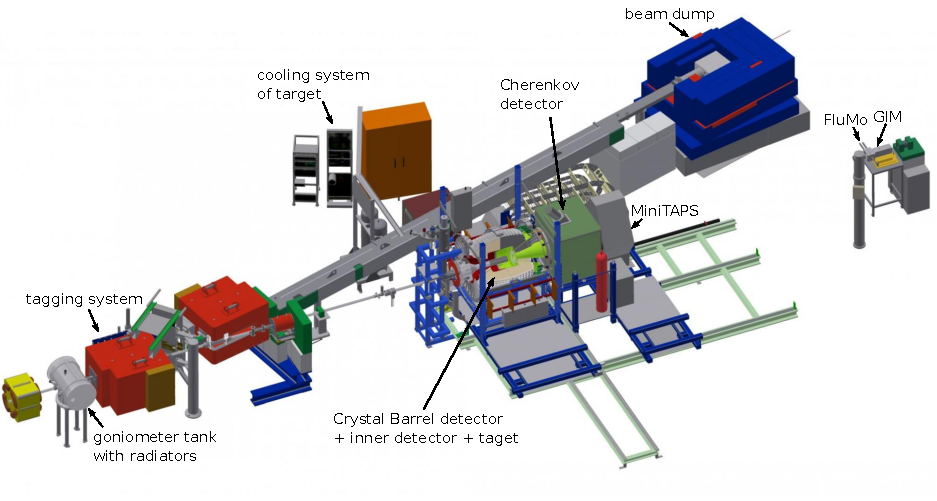
\includegraphics[width=\linewidth]{figs/cbarea.pdf}
	\caption{Overview of the experimental hall of the CBELSA/TAPS experiment. The electron beam from ELSA enters at the top right. \textsc{M. Grüner} in \cite{farahphd}}
	\label{fig:cbarea}
\end{figure}
\noindent High energy electrons extracted from ELSA are used to produce a polarized photon beam using the \emph{bremsstrahlung} process (see \ref{subsec:goni}). After they have been energy tagged (see \ref{subsec:tag}) these photons then interact with the fixed target material (see Section \ref{sec:tar}) so that hadronic resonances may be excited that will decay via the strong interaction under the emission of mesons. The resulting decay products can then be measured with a system of electromagnetic calorimeters and scintillators that is especially suited for the detection of photons (see Section \ref{sec:cal}). The analogue measurements are only saved for offline analysis if detector signals meet certain trigger conditions which is only the case for reactions that are of interest (see Section \ref{sec:trig}). This way the amount of unwanted background is minimized already during the process of data taking. Once data acquisition is finished the data may be investigated with the help of analysis software and Monte Carlo simulations tailored to the needs of the CBELSA/TAPS experiment (see Section \ref{sec:mc}).
\section{Production of polarized high energy photon beam}
\label{sec:pol}
To measure polarization observables in photoproduction reactions a polarized photon beam is needed which can be created using \emph{coherent bremsstrahlung}. Bremsstrahlung is the dominating interaction of high energy ($\mathcal{O}\left(\SI{1e0}{\giga\eV}\right)$) electrons with matter \cite{leo}. Electrons are decelerated in the \textsc{Coloumb} field of heavy nuclei and radiate real photons, see Figure \ref{fig:brems}. 

\begin{figure}[htbp]
	\centering
	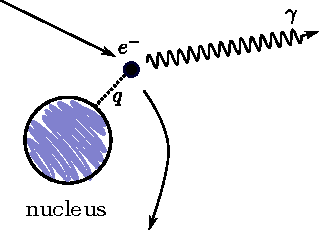
\includegraphics[width=.5\linewidth]{brems.pdf}
	\caption{Illustration of the bremsstrahlung process: An electron $e^-$ is deflected in the \textsc{Coloumb} field of a nucleus in the radiator material. A photon $\gamma$ is emitted and so the momentum $q$ is transferred.}
	\label{fig:brems}
\end{figure}
\noindent To conserve momentum there has to be a momentum transfer $q$ which is negligibly small compared to the nucleon mass. If an amorphous radiator is used incoherent bremsstrahlung is produced with a continuous spectral distribution proportional to $1/E_\gamma$ according to the \textsc{Bethe-Heithler} cross section \cite{hei}. Since the structure of nuclei in the amorphous radiator does not exhibit any periodicity, the electric field vector will not prefer any particular direction, resulting in a net polarization degree of zero for the photon beam. To achieve non-vanishing polarization degrees a crystal with periodic placement of nuclei may be used as radiator. Then, coherent bremsstrahlung is produced; the crystal can absorb the recoil only for discrete momenta $q_n$ meeting the \textsc{Laue} condition \cite{dem} of the crystal lattice. This enables constructive interference between different bremsstrahl photons and at the same time fixes the deflection plane of incoming electrons, resulting in a coherent polarized photon beam. Incoherent bremsstrahlung may still occur due to impurities in the crystal structure, so that the total bremsstrahlung cross section off a crystal radiator $\sigma_\text{crystal}$ is the sum of a coherent ($\sigma_\text{coherent}$) and an incoherent ($\sigma_\text{incoherent}$) part
\begin{equation}
	\sigma_\text{crystal}=\sigma_\text{coherent}+\sigma_\text{incoherent}.
\end{equation}
The process of bremsstrahlung can be modeled using ANalytical Bremsstrahlung (ANB) calculations \cite{anb}. ANB intensity spectra for a crystal and amorphous radiator are shown in Figure \ref{fig:anb} on the left hand side. The right hand side shows the enhancement spectrum, which is given by dividing the two spectra. 
\begin{figure}[htbp]
	\centering
	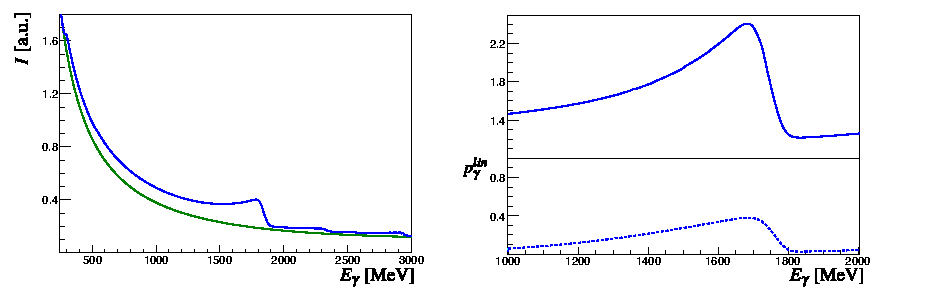
\includegraphics[width=\linewidth]{figs/anb.pdf}
	\caption{Left: Incoherent (green) and crystal (blue) bremsstrahlung intensities as a function of the photon energy. Right: The enhancement spectrum is given as the ratio of crystal to incoherent intensity spectrum. The dashed line at the bottom shows the calculated polarization degree. Both spectra are generated using ANB calculations. Taken from \cite{farahphd}.}
	\label{fig:anb}
\end{figure} 
One observes that the bremsstrahlung intensity spectrum obtained from a crystal radiator is in general enhanced relative to the incoherent spectrum obtained from an amorphous radiator. In fact, using ANB calculations, the polarization degree can be determined from the enhancement spectrum. The characteristic drop in intensity in the intensity spectrum obtained from the crystal radiator is referred to as the coherent edge. It occurs because the photon energy in the kinematically allowed region of the recoil momentum that will lead to coherent bremsstrahlung is limited. The relative alignment of the radiation crystal to the electron beam determines the position of the coherent edge. 
\subsection{Goniometer}
In order to determine the beam polarization from enhancement spectra, a diamond radiator as well as an amorphous radiator are required. Several radiators as well as beam diagnostics tools mounted inside a rotating aluminum wheel are part of the goniometer \cite{goni}, resting inside a vacuum tank. Depending on whether linearly polarized or unpolarized photons are needed either copper radiators of different thickness or a diamond radiator, which is located in the center of the wheel, are inserted into the beam axis, see Figure \ref{fig:goni}. In case a circularly polarized photon beam is required, a \textsc{M\o ller} polarimeter \cite{moller} is used, which is also shown in Figure \ref{fig:goni}. The goniometer can be rotated in all directions allowing precise alignment with the incoming electron beam from ELSA.  
\label{subsec:goni}

\subsection{Tagging system}
\label{subsec:tag}
Once the impinging electrons from ELSA have scattered off the radiator their energy is determined in order to measure the energy of the created photons. This is possible because the initial electron energy $E_0=\SI{3.2}{\giga\eV}$ is known from ELSA. Thus, the photon Energy $E_\gamma$ is given by subtracting the energy of the recoil electrons $E_e$ from $E_0$\footnote{Hereby, the recoil energy absorbed by the nuclei is neglected.} 
\begin{equation}
	E_\gamma=E_0-E_e.
\end{equation}
The recoiling electrons are deflected towards the tagging system \cite{tagger} consisting of 96 overlapping scintillator bars and 480 scintillating fibers using the magnetic field of a dipole magnet with a field strength of $\SI{1.5}{\tesla}$. The bending radius of the electrons depends on their momenta is uniquely defined by the tagger hit position. With the position of the deflected electrons and the magnetic field strength, $E_e$ can thus be determined. For an initial energy $E_0=\SI{3.2}{\giga\eV}$ the scintillator bars cover an energy range of $\SI{560}{\mega\eV}<E_\gamma<\SI{3100}{\mega\eV}$ with an energy resolution of $0.1\%E_\gamma$-$6\%E_\gamma$. The fibers additionally improve the energy resolution in the energy range $\SI{416}{\mega\eV}<E_\gamma<\SI{2670}{\mega\eV}$ to $0.1\%E_\gamma$-$0.4\%E_\gamma$. Photomultipliers are used for the readout of the tagger bars and fibers, realizing a time resolution of \footnote{Full Width Half Maximum.}$\text{FWHM}_\text{bar}=\SI{635}{\pico\s}$ and $\text{FWHM}_\text{fiber}=\SI{1.964}{\nano\s}$ \cite{hartmanndipl}. Any electrons that have not interacted with the radiator material are deflected by another dipole magnet towards the beam dump, see Figure \ref{fig:cbarea}. Figure \ref{fig:tagger} shows a top-down view of the tagging system.

\begin{minipage}[htbp]{.45\linewidth}
	\begin{figure}[H]
		\centering
		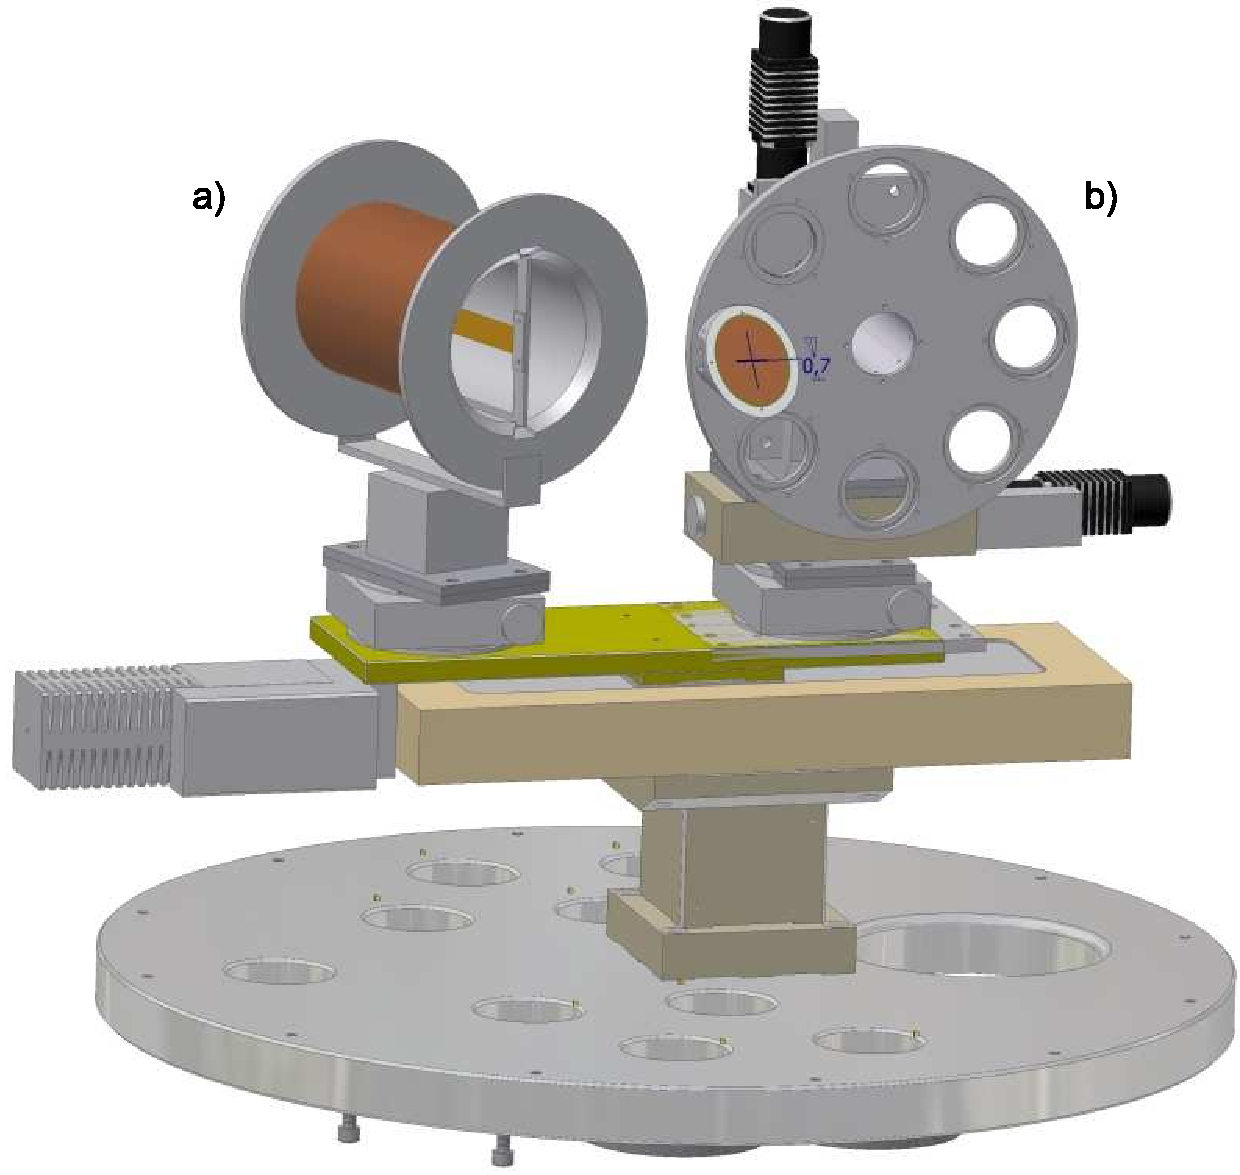
\includegraphics[width=\linewidth]{figs/goni-ganz.pdf}
		\caption{The goniometer holds several radiators that can be inserted onto the beam axis (b). Also available is a \textsc{M\o ller} radiator \cite{cb}.\\}
		\label{fig:goni}
	\end{figure}
\end{minipage}
\hfill
\begin{minipage}[htbp]{.49\linewidth}
\begin{figure}[H]
	\centering
	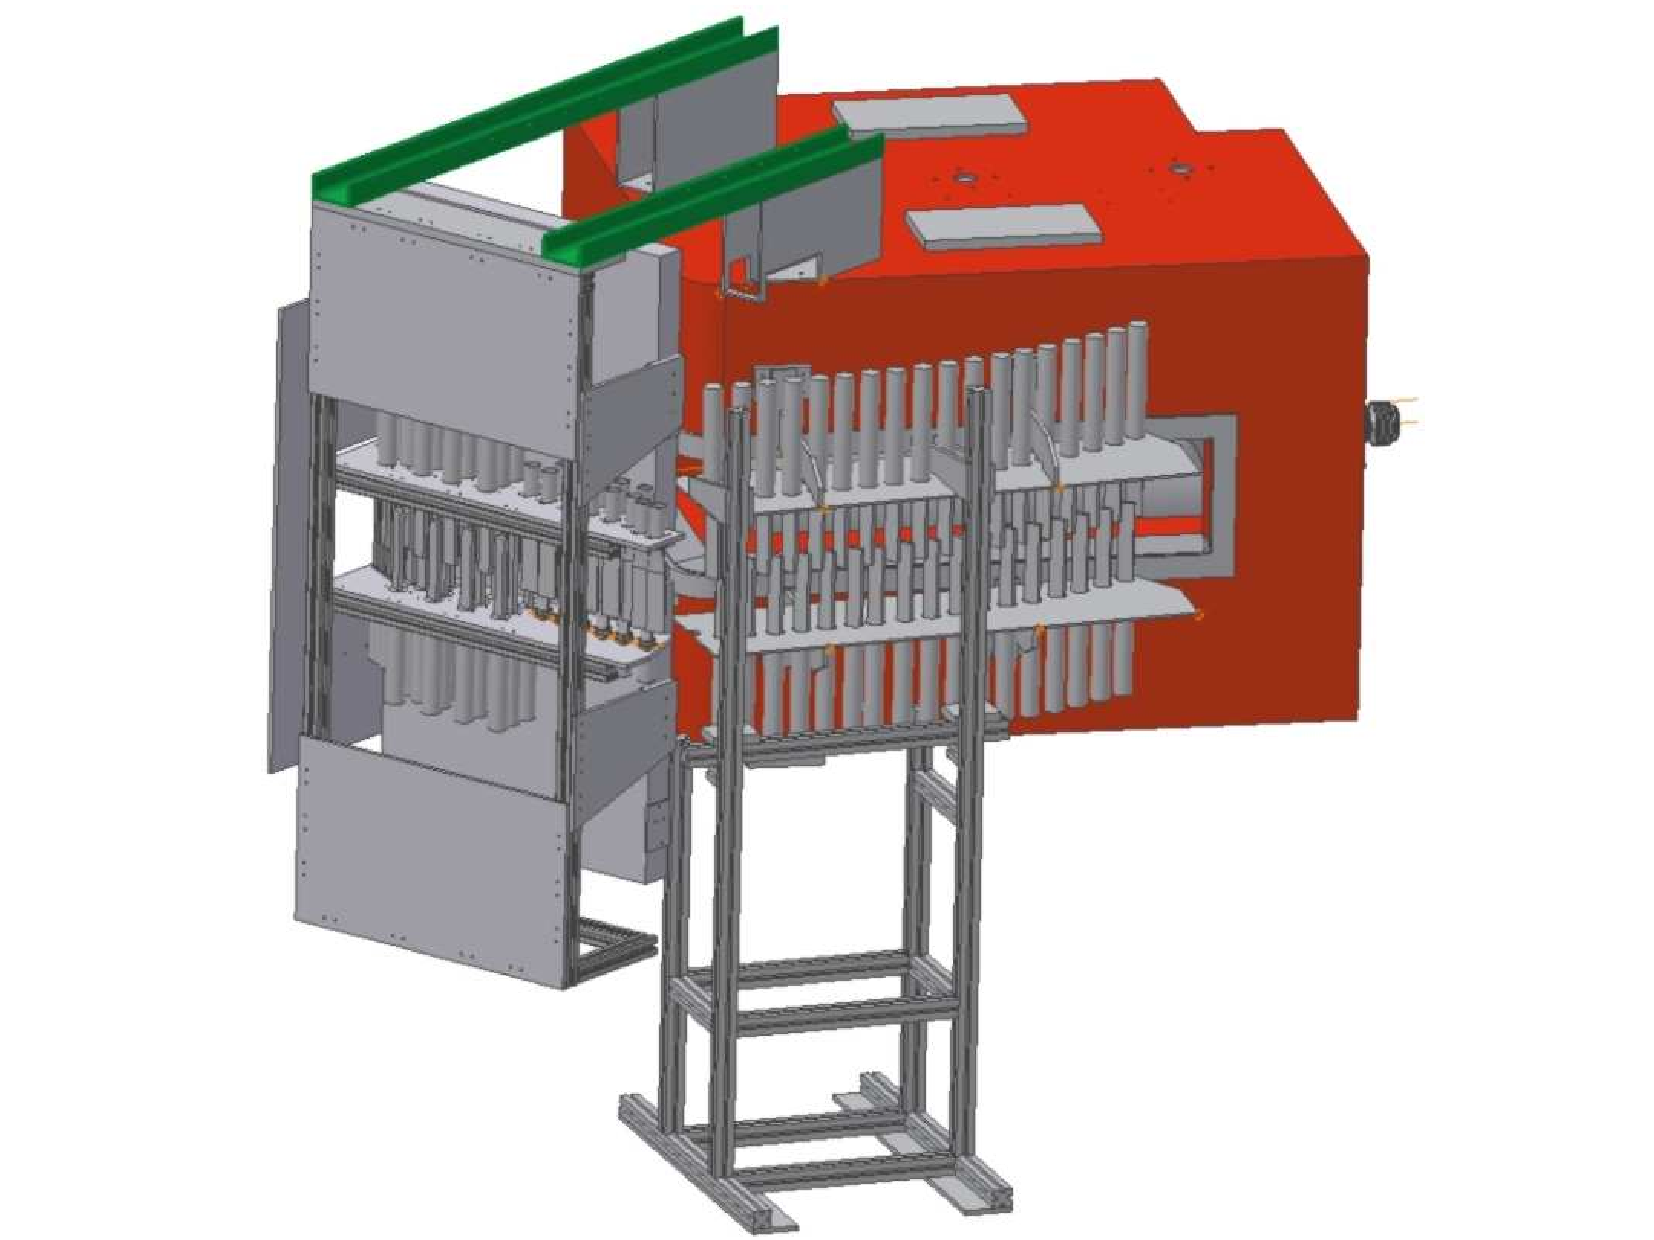
\includegraphics[width=\linewidth]{figs/Tagger.pdf}
	\caption{Top-down view of the tagging system consisting of dipole magnet (red) and scintillating bars and fibers \cite{tagger}. Electrons are deflected by the magnet after the bremsstrahlung process.}
	\label{fig:tagger}
\end{figure}
\end{minipage}
\section{Liquid hydrogen target}
\label{sec:tar}
The (polarized) photon beam impinges on a liquid hydrogen target \cite{hammannphd} which is located at the center of the crystal barrel detector, see Figure \ref{fig:cbarea}. It consists of a Kapton cell that measures $\SI{5.1}{\centi\m}$ in length and $\SI{3}{\centi\m}$ in diameter which is filled with liquid hydrogen. A separate cooling circuit with liquid hydrogen ensures the hydrogen that is used as target material stays liquid. Kapton is chosen as material for the target cell because the expected rate of hadronic reactions induced in the target cell is small compared to the expected rate from liquid hydrogen \cite{hammannphd}. Protons are bound with a binding energy of $\SI{21.4}{\eV}$ in the target material, which is negligible on the scale of hadronic reaction energies, so that they can be considered free. A schematic view of the target is shown in Figure \ref{fig:target}.
\begin{figure}[htbp]
	\centering
	\includegraphics[width=\linewidth]{figs/Target.pdf}
	\caption{Schematic overview of the liquid hydrogen target. Two tubes connected to a heat exchanger and the Kapton cell allow filling it with liquid hydrogen. \textsc{M. Grüner} in \cite{farahphd}.}
	\label{fig:target}
\end{figure}
\section{Detector system}
\label{sec:cal}
Hadronic reactions are induced by the photon beam in the target material. As a consequence resonances are excited that decay under emission of mesons. These mesons subsequently decay to e.g. photons. The main calorimeters of the experiment, the Crystal Barrel that is complemented by the forward detector(\ref{sec:cb}) and the MiniTAPS calorimeter (\ref{sec:mt}), cover $95\%$ of the solid angle $4\pi$ and are especially suited for the detection of photons. Charged particles are identified by the inner detector (\ref{sec:in}) as well as plastic scintillators mounted in front of the forward and the MiniTAPS detector that are used as vetoes. To suppress electromagnetic reactions a \textsc{\v Cerenkov} detector is used (\ref{sec:cerenkov}). The photon flux is measured via the Gamma-Intensity-Monitor (GIM) and Flux-Monitor (FluMo) (\ref{sec:flumo}).
\subsection{Inner detector}
\label{sec:in}
The inner detector \cite{indet,suft} encloses the target in a cylindrical geometry and consists of 513 plastic scintillation fibers that are placed in three layers. The outer layer is oriented along the beam axis while the inner layers are tilted by an angle of $\SI{-24.5}{\degree}$ and $\SI{25.8}{\degree}$, respectively, see Figure \ref{fig:indet}.
\begin{figure}[htbp]
	\centering
	
\includegraphics[width=\linewidth]{figs/indet.pdf}
	\caption{The inner detector with three layers of scintillating fibers. The inner two layers are tilted with respect to the outer layer. \textsc{D. Walther} in \cite{farahphd}.}
	\label{fig:indet}
\end{figure}
This structure allows to determine the azimuthal and polar angle of a charged particle as long as at least two layers are hit. The detector is in total $\SI{40}{\centi\meter}$ long and covers a polar angle range of $\SI{23.1}{\degree}<\theta<\SI{166}{\degree}$ with a resolution of $\SI{0.4}{\degree}$ in polar angle $\theta$ and $\SI{0.1}{\degree}$ in azimuthal angle $\phi$. The fibers consist of Polystyrene with a refractive index of $n=1.6$ and are cladded by Polymethylmetacrylat ($\text{C}_5\text{H}_8\text{O}_2$) with $n=1.49$ \cite{prop}. Charged particles passing the detector will cause the emission of scintillation light by the Polystyrene molecules which is read out with photomultipliers after passing lightguides. Short decay times ensure a fast time signal and a time resolution of $\text{FWHM}=\SI{2.093\pm0.013}{\nano\s}$ is reached \cite{hartmanndipl}.
\subsection{Crystal Barrel and forward detector}
\label{sec:cb}
The main calorimeter of the experiment is the Crystal Barrel detector \cite{cbdet}. It consists of 1320 CsI(Tl) crystals that are arranged in 24 rings facing the center of the target, see Figure \ref{fig:cb}.
\begin{figure}[htbp]
	\centering
	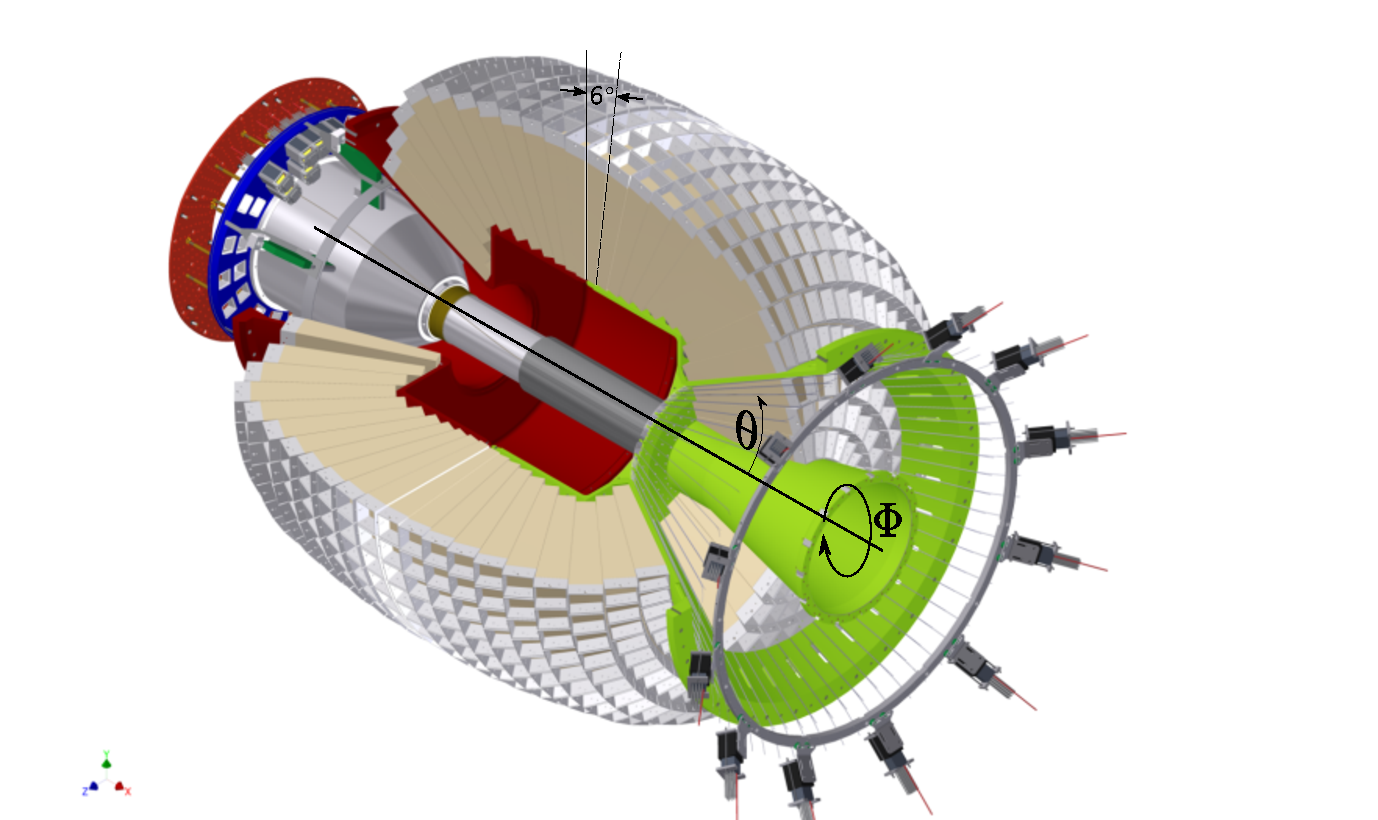
\includegraphics[width=\linewidth]{figs/cb_fp_in.pdf}
	\caption{Crystal barrel calorimeter and forward detector are built such that they enclose the target and the inner detector. The forward detector consists of the first three rings (green base) of crystals which are additionally covered by plastic scintillators for charged particle identification. The definition of polar angle $\theta$ and azimuthal angle $\phi$ in the LAB system are indicated as well.\textsc{D. Walther} in \cite{urban}}
	\label{fig:cb}
\end{figure} The first three rings in forward direction contain 30 crystals each and build the forward detector, covering the polar angle range $\SI{11.18}{\degree}<\theta<\SI{27.54}{\degree}$. Also the $24^\text{th}$ ring contains 30 crystals, all other rings are made up of 60 crystals. The crystals are shaped like truncated trapezoidal pyramids that cover $\SI{6}{\degree}$ in polar angle $\theta$ and azimuthal angle $\phi$. Only in the first three and the last ring the crystals cover $\SI{12}{\degree}$ in $\phi$. Full coverage in $\phi$ and $80\%$ ($\SI{12}{\degree}<\theta<\SI{156}{\degree}$) coverage in $\theta$ are achieved by the forward detector and the Crystal Barrel. Photons from neutral mesonic decays are very high energetic and will interact with the inorganic scintillator material mainly via pair production \cite{leo}. The produced electrons and positrons will themselves interact mainly via bremsstrahlung such that usually an electromagnetic shower is created upon photon impact that may spread over several crystals. Using crystals with a length of $l=\SI{30}{\centi\meter}$ photons with an energy of up to $\SI{2}{\giga\eV}$ may deposit their entire energy in the calorimeter since the $l$ corresponds to $16.22$ radiation lengths $X_0$ \cite{cbdet}. The transversal spread of a shower is given by the \textsc{M\'oliere} radius which is $\SI{3.8}{\centi\meter}$ for CsI(Tl) \cite{cbdet}. By determining the focal point of the electromagnetic showers an angular resolution of less than $\SI{2}{\degree}$ can be achieved \cite{cbang} while the energy resolution is given by \cite{cbdet}
\begin{equation}
	\frac{\sigma_E}{E}=\frac{2.5\%}{\sqrt[4]{E/\si{\giga\eV}}},
\end{equation}
depending on the initial photon energy $E$. The energy loss of heavier charged particles, e.g. a proton, is described by the \textsc{Bethe-Bloch} formula \cite{bethe}. Depending on their mass they only deposit their full energy up to a certain threshold energy above which they are characterized as Minimal Ionizing Particles (MIP).

The emitted scintillation light of crystals not belonging to the forward detector is read out using PIN photodiodes. A wavelength shifter ensures meeting the sensitive spectral range of the photodiodes. The long decay times of the scintillation light and the slow preamplifiers following the photodiodes do not allow the determination of a timing information for particles detected in the Crystal Barrel \footnote{As of 2014, the PIN photodiodes have been replaced by avalanche photodiodes (APD) \cite{honisch,urban}, allowing a fast read out that can be used to provide timing information and also as part of the trigger.}, so that the Crystal Barrel is optimized for energy measurements.

Crystals belonging to the forward detector are read out using Photomultipliers. They provide a faster signal, such that timing information for forward detector hits is available with a time resolution of $\text{FWHM}=\SI{1.861\pm0.016}{\nano\s}$ \cite{hartmanndipl}. Additionally plastic scintillator plates are mounted in front \cite{wendel}, allowing the identification of charged particles with an efficiency of $72\%$ \cite{fw}. Optical fibers guide the scintillation light from the plates to photomultipliers.
\subsection{MiniTAPS}
\label{sec:mt}
Since the Crystal Barrel only covers the solid angle starting at $\theta\approx\SI{12}{\degree}$. It is supplemented by the Mini-Two-Arm-Photon-Spectrometer (MiniTAPS) \cite{mt1,mt2} for polar angles $\SI{1}{\degree}<\theta<\SI{12}{\degree}$. The MiniTAPS detector is placed in a distance of $d=\SI{2.1}{\m}$ from the target and consists of 216 hexagonally shaped BaF$_2$ crystals, see Figure \ref{fig:minitaps}. Each crystal has a length of $l=\SI{25}{\centi\m}$ which is equivalent to 12 radiation lengths \cite{mtrad} and a width of $w=\SI{5.8}{\centi\meter}$. The chosen material has a high density and is able to withstand high reaction rates \cite{prop}. This is important here because most reactions will be strongly boosted in forward direction towards small $\theta$. Different mechanisms of scintillation allow to extract a fast and a slow component \cite{leo} which are read out using photomultipliers and separately used for timing and energy information, respectively. Hereby a time resolution of $\text{FWHM}=\SI{0.872\pm0.006}{\nano\s}$ \cite{hartmanndipl} and an energy resolution of \cite{mt1} \begin{equation}
	\frac{\sigma_E}{E}=1.9\%+0.59\%\cdot\sqrt{E/\si{\giga\eV}}
	\end{equation}
is achieved. At the same time an angular precision of $\SI{0.2}{\degree}$ in $\theta$ is reached. 

In front of each BaF$_2$ crystal, plastic scintillator plates are mounted to identify charged particles. Their scintillation light is guided towards photomultipliers using optical fibers. With these scintillators a time resolution of $\text{FWHM}=\SI{3.06\pm0.05}{\nano\second}$ is obtained \cite{hartmanndipl}. 
\begin{figure}[htbp]
	\centering
	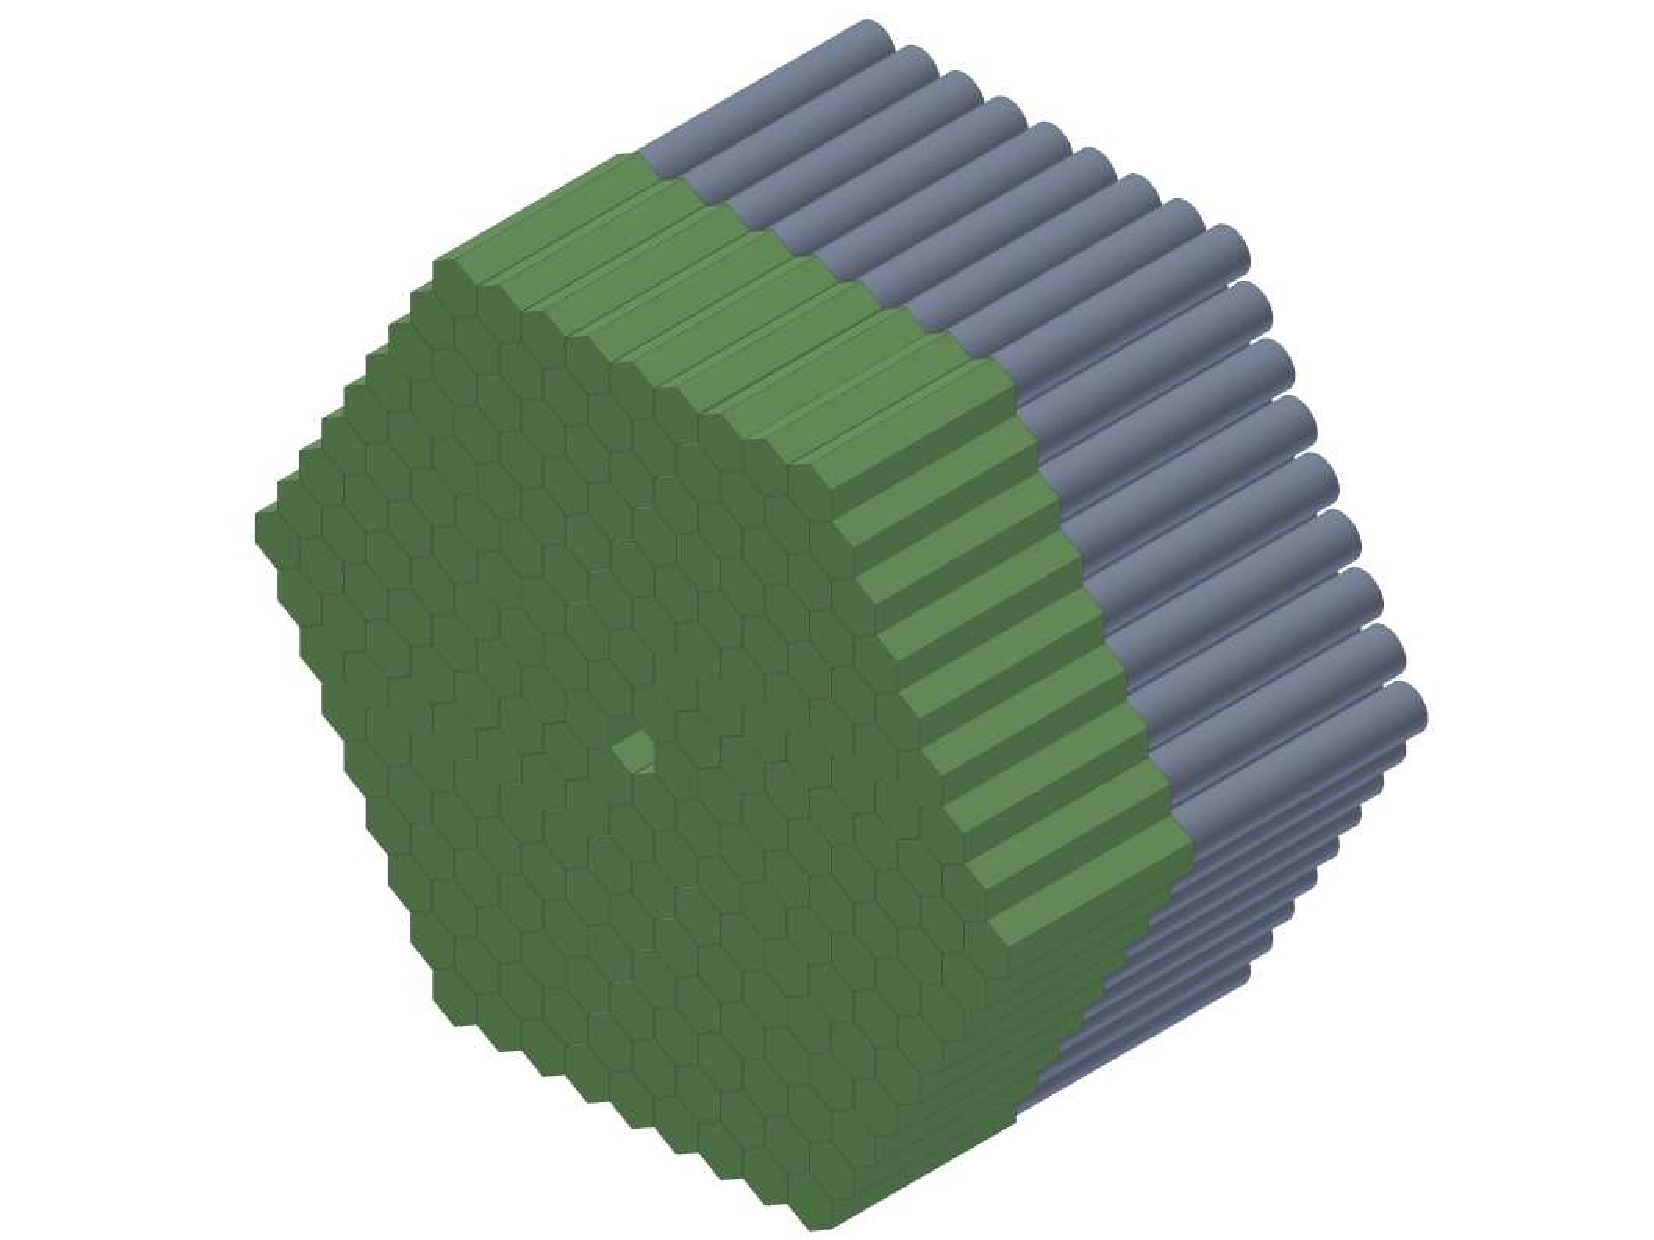
\includegraphics[width=.5\linewidth]{figs/mini-taps.pdf}
	\caption{The MiniTAPS detector is made up of 216 BaF$_2$ crystals (grey). In front of each crystal, plastic scintillators are mounted for charged particle information. Taken from \cite{cb}.}
	\label{fig:minitaps}
\end{figure}
\subsection{\textsc{\v Cerenkov} detector}
\label{sec:cerenkov}
When the photon beam impinges on the proton target, not only hadronic reactions are induced but also electromagnetic reactions. Because the beam energy is very high on the scale of electromagnetic interactions, any produced electrons and positrons are highly relativistic and boosted to small polar angles. To suppress these events already during data acquisition a \textsc{\u Cerenkov} detector \cite{cerenkov} is positioned between the MiniTAPS calorimeter and the Crystal Barrel, see Figure \ref{fig:cbarea}. It is filled with CO$_2$ gas where \textsc{\v Cerenkov} light is emitted by electrons or positrons above an energy of $\SI{17.4}{\mega\eV}$. This follows from the refractive index which is given as $n_{\text{CO}_2}=1.00045$ \cite{prop}. The emitted \textsc{\u Cerenkov} radiation is focused on a photodiode using a parabolic mirror. The presence of a signal can then be used as veto during data acquisition to reduce the amount of recorded electromagnetic background. Electrons and positrons are detected with an efficiency of up to $(99.72\pm0.45)\%$ \cite{cerenkov}.
\subsection{Flux monitoring}
\label{sec:flumo}
The FluMo and GIM detector are used to determine the total number of photons incident on the target and are located behind the MiniTAPS detector, as is shown in Figure \ref{fig:cbarea}.

The GIM detector \cite{gim} is made of 16 PbF$_2$ crystals placed in a $4\times4$ array, see Figure \ref{fig:gim}. Incoming photons will interact with the material mainly via pair production \cite{leo}. The produced electrons and positrons are highly relativistic and will emit \textsc{\v Cerenkov} light that is collected with photomultipliers. For reaction rates higher than $\SI{5}{\mega\Hz}$ the GIM detector efficiency decreases significantly. For rates above $\SI{7}{\mega\Hz}$ more than $10\%$ of events are not registered \cite{hartmanndipl}. 
\begin{figure}[htbp]
	\centering
	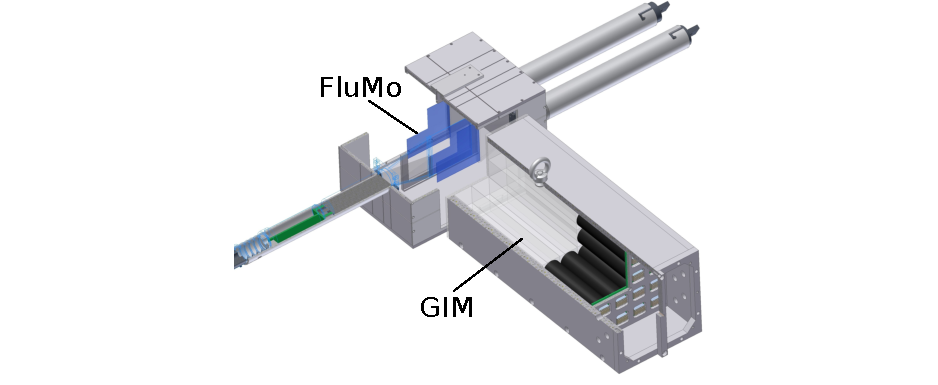
\includegraphics[width=\linewidth]{flumo.pdf}
	\caption{The two detectors FluMo and GIM are used to monitor the photon flux at different reaction rates. \textsc{D. Walther} in \cite{farahphd}.}
	\label{fig:gim}
\end{figure}  
To compensate this the FluMo detector \cite{flumo} is used as soon as deadtime effects influence the performance of the GIM detector. A converter plate made of lead, two scintillators and a veto detector are part of the FluMo detector. Impinging photons may create electron positron pairs that are detected in a coincidence measurement using the two scintillators. A plastic scintillation detector is placed before the converter plate and gives a veto signal if charged particles pass through it.

\section{Trigger}
\label{sec:trig}
To minimize the volume of data that is saved to disk for offline analysis, data is only digitized if certain predefined patterns in the detector signals are present. The search for predefined patterns is managed by the trigger of the experiment. The analyzed data sets were acquired using the \emph{vme\_trig42c} trigger \cite{trig1,trig2}. The trigger requires configuration to be sensitive to hadronic photoproduction reactions and at the same time reject unwanted background events. This is achieved using Field Programmable Gate Arrays (FPGAs) which allows to split the trigger into two levels: At first level all detectors with a fast read out system (up to \SI{250}{\nano\s}) are checked for hits. At the second level the number of detected particles in the Crystal Barrel is determined using the Fast Cluster Encoder (FACE), which can take up to $\SI{10}{\micro\s}$ \cite{face}. It is always demanded that at least two particles are measured in either forward, MiniTAPS or Crystal Barrel detector while no veto from the \textsc{\v Cerenkov} detector is measured. Any information from the Crystal Barrel is only available in the second level because of the slow readout.
\section{Software and Monte Carlo}
\label{sec:mc}
In order to proceed with the offline data analysis of CBELSA/TAPS, several software tools are used that are described briefly in the following.
\subsection{ExPLORA}
Within the CBELSA/TAPS collaboration an analysis software has been developed named \emph{Extended Pluggable Object-oriented Root Analysis (ExPLORA)} \cite{explora}. It is based on \emph{ROOT} \cite{root} and is used for reconstruction and analysis of acquired raw data. \emph{ROOT} has been developed at CERN to deal with a high amount of data. It makes use of \emph{C++} libraries that give it high funcitonality regarding statistical analyses, visualizations and data management. \emph{ExPLORA} is also written in \emph{C++} but is operated by the use of \emph{xml} files. This allows user specific extensions in the form of plugins that manage e.g. the application of cuts and the filling of histograms. In order to select candidates for the reaction $\gamma p\to p\eta'\to p\gamma\gamma$ a \emph{C++} plugin has been written that was embedded into a \emph{xml} file which managed the application of calibrations and reconstruction. For further anaylsis of the selected data, scripts in \emph{ROOT} and \emph{python} have been written. In Appendix \ref{app:soft} an example \texttt{.xml} file is displayed.
\subsection{Monte Carlo}
In order to determine detector and analysis acceptances as well as possible background contributions it is convenient to simulate the according detector geometry and the interaction of particles with the material using the Monte Carlo technique \cite{mc}. Based on the CERN-developed software package \emph{Geant3} (Geometry and Tracking) \cite{g3} a simulation of the CBELSA/TAPS experiment was developed using the Virtual Monte Carlo technique \cite{kalisch}. Hereby the particles' interaction with the detector materials are modeled according to existing experimental data. Simulated datasets may then be analyzed in the same way as measured data in order to check consistency with the measured data as well as investigating detection efficiencies and background contributions. Table \ref{tab:mc} shows the simulated datasets that were used during the analysis and how many events were generated for each reaction, respectively. The reactions $\gamma p\to p2\pi^0\to p4\gamma$ $\gamma p\to p\pi^0\eta\to p4\gamma$ proved to be responsible for background contamination after the event selection (see Chapter \ref{chap:events}). These reactions were simulated while additionally weighting all events according to the production cross section determined from a BnGa fit \cite{bnga1,bnga2}.  These Monte Carlos were kindly provided by \textsc{P. Mahlberg} \cite{mahlbergphd}.
\begin{table}[htbp]
	\centering
	\begin{tabular}{cc}
		\toprule
		Reaction & Number of events\\
		\hline
		$\gamma p \to p\pi^0$ & $60\cdot10^6$\\
		$\gamma p \to p\eta$ & $30\cdot10^6$\\
		$\gamma p \to p\omega\to p\pi^0\gamma$ & $30\cdot10^6$\\
		$\gamma p \to p\eta'\to p\gamma\gamma$ & $30\cdot10^6$\\
		$\gamma p \to p2\pi^0$ & $60\cdot10^6$\\
		$\gamma p \to p\pi^0\eta$ & $60\cdot10^6$\\
		$\gamma p \to p3\pi^0$ & $30\cdot10^6$\\
		$\gamma p \to p2\pi^0\eta$ & $30\cdot10^6$\\
		$\gamma p \to n\pi^+$ & $30\cdot10^6$\\
		$\gamma p \to p\pi^+\pi^-$ & $30\cdot10^6$\\
		\bottomrule
	\end{tabular}
\end{table}
\subsection{Stan}
All \textsc{Bayesian} fits that are presented in this thesis are performed using the progamming language \emph{Stan} \cite{stan}. \emph{Stan} is highly functional for statistical modeling and high-performance statistical computation. Full \textsc{Bayesian} statistical inferences can be made with MCMC sampling as well as approximate \textsc{Bayesian} inference with variational inference and penalized maximum likelihood estimation with optimization \cite{stan}. Stan is written in \emph{C++} and can thus handle a large amount of data very efficiently. Interfaces for different data analysis languages are available. In this thesis, the \emph{Python} \cite{python} front-end of \emph{Stan}, called \emph{CmdStanPy} was used. Hereby, the model is specified in a \texttt{.stan} file which is read and compiled from \emph{Python}. All sampling statements and results can then be accessed directly from \emph{Python}, e.g. using the package \texttt{pandas} \cite{pandas}. Appendix \ref{app:soft} shows an example of a \texttt{.stan} file that can be used for the simple example of a linear fit.
\section{Datasets}
The data that was analyzed in the course of this thesis was taken in the period of July 2013 to October 2013. Unpolarized electrons from ELSA were incident on a diamond radiator with $\SI{500}{\micro\meter}$ thickness with a beam energy of $E_0=\SI{3.2}{\giga\eV}$ and a beam current of roughly $\SI{1}{\nano\ampere}$. Thus, linearly polarized photons were created that impinged on a liquid hydrogen target. All beam times used the \emph{vme\_trig42c} that has been described previously.

The coherent edge position was chosen at $\SI{1750}{\mega\eV}$ for the July and August beam times and at $\SI{1850}{\mega\eV}$ for the September and October beam times, enabling an analysis of the beam asymmetry $\Sigma$ in the beam energy range from $E_\gamma\approx\SI{1100}{\mega\eV}$ to $\SI{1800}{\mega\eV}$.  4919 runs were taken in total  with alternating radiator orientation $\alpha^{\parallel/\bot}=\SI{45}{\degree}$, see Figure \ref{fig:angles}. The photon beam polarization was determined as part of the work \cite{farahphd} using ANB calculations, as described in Section \ref{sec:pol}. Table \ref{tab:sumbeam} shows a summary of the key parameters of the 2013 beam time taken at the CBELSA/TAPS experiment.

\begin{table}[htbp]
	\centering
	\begin{tabular}{ccc}
		\toprule
\textbf{beamtime} & \textbf{number of runs (h)} & \textbf{coherent edge position}\\
\hline
July 2013 & 513 (111) & \SI{1750}{\mega\eV}\\	
August 2013 & 1832 (396) & \SI{1750}{\mega\eV}\\		
September 2013 & 1490 (323) & \SI{1850}{\mega\eV}\\		
October 2013 & 1084 (235) & \SI{1850}{\mega\eV}\\			
\bottomrule
\end{tabular}
\caption{Summary of the key parameters of the 2013 beam time at CBELSA/TAPS taken for the measurement of the beam asymmetry $\Sigma$. Taken from \cite{farahphd}.}
\label{tab:sumbeam}
\end{table}



